\newpage

\section{Вычислительный эксперимент}
\subsection{Данные} 
Открытый исходный датасет для мультиклассовой классификации текстов, написанных человеком и различными языковыми моделями~\cite{semeval2024task8}. Изначально было представлено 6 классов (включая человека), но из-за технических ограничений количество классов было сокращено до 4: ChatGPT, Davinci, Cohere, Humans. Всего в датасете 21 000 текстов с разметкой по классам.

\subsection{Предобработка}
Тексты были токенизированы при помощи AutoTokenizer~\cite{wolf2019huggingface}. Дополнительная обработка не требуется из-за структуры модели~\cite{vaswani2017attention}.

\subsection{Эксперименты} 
Для всех экспериментов использовалась предобученная модель DistilRoBERTa base (далее в тексте - DRoBERTa-base)~\cite{liu2019roberta}. Модель использовалась со следующими гиперпараметрами: доля тренировочного/тестового набора данных - 0.9/0.1; 3 эпохи обучения. Для экспериментов с использованием алгоритма LoRA были использованы все вышеуказанные параметры, а также ранг матриц аппроксимации r = 5.

\newpage
\subsection{Эксперимент (1)}
\textbf{Предобученная модель DRoBERTa-base обучилась на всем обучающем датасете.}\\ \\
После обучения для оценки использовались матрица ошибок и метрики точности, полноты и F1-меры: \newline
\textbf{train\_runtime: 4041.3188}
\begin{figure}[h]
    \centering
    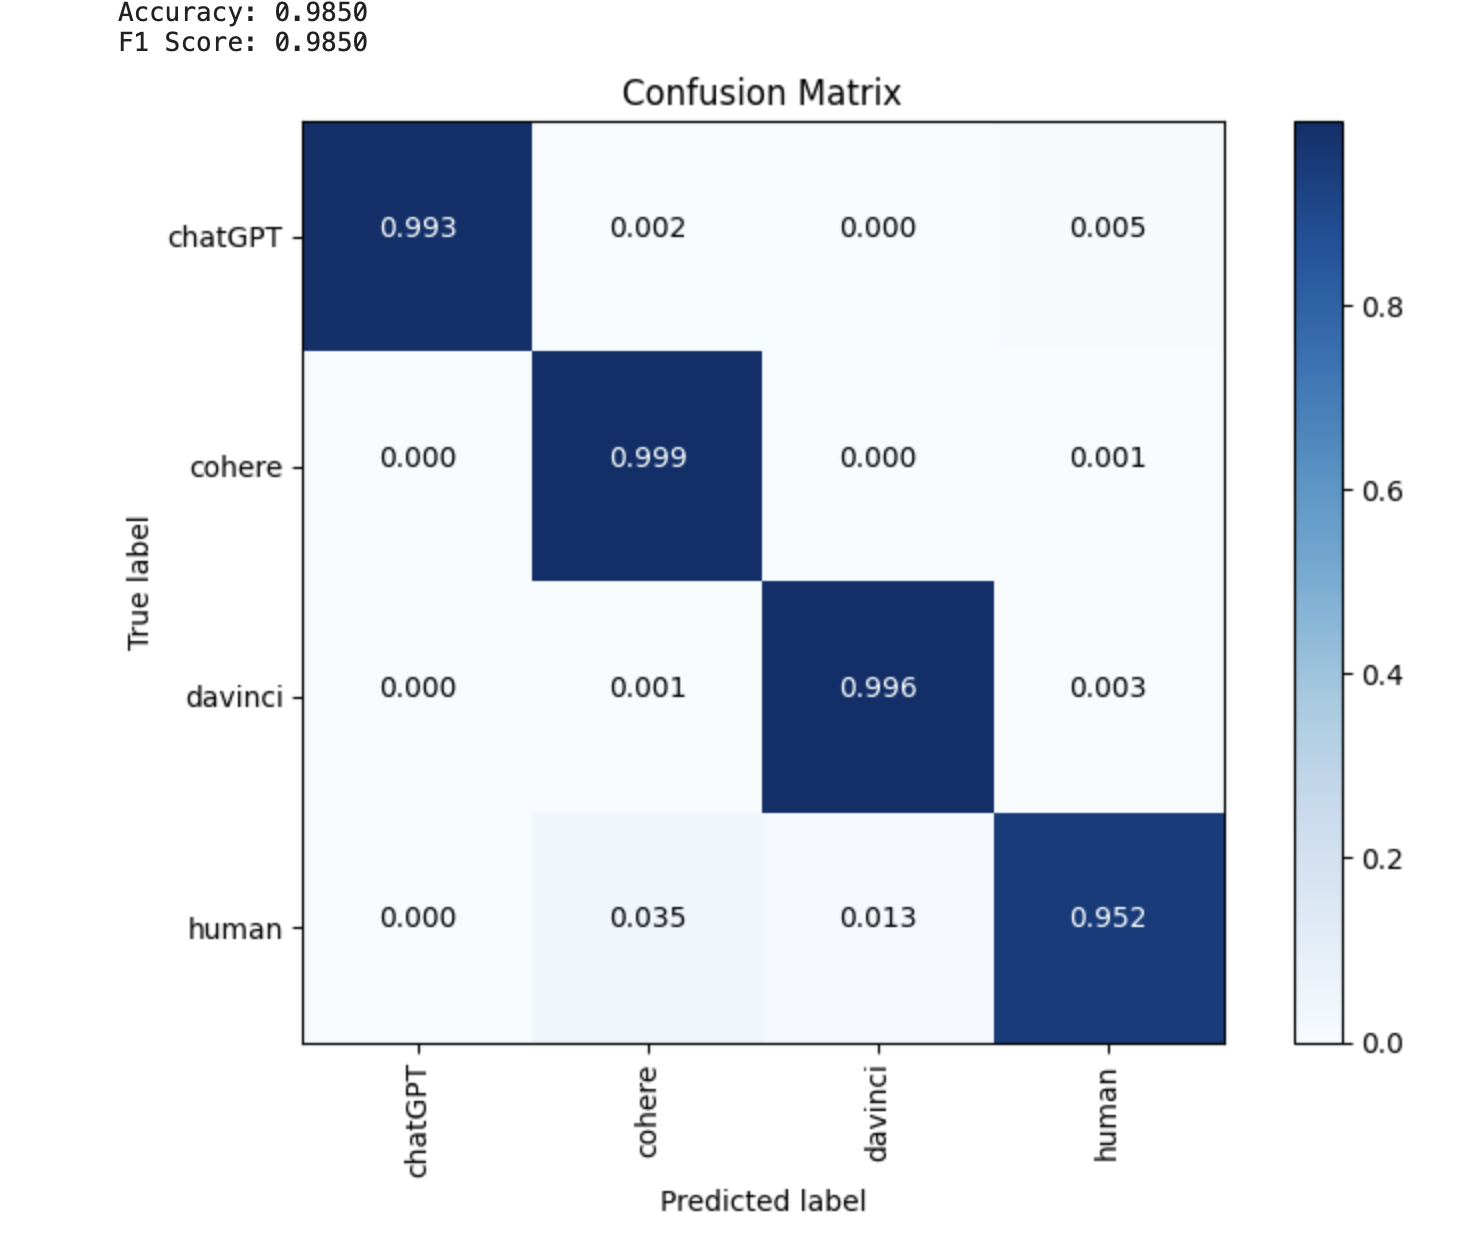
\includegraphics[width=.75\textwidth]{images/bert_vanilla.png}
    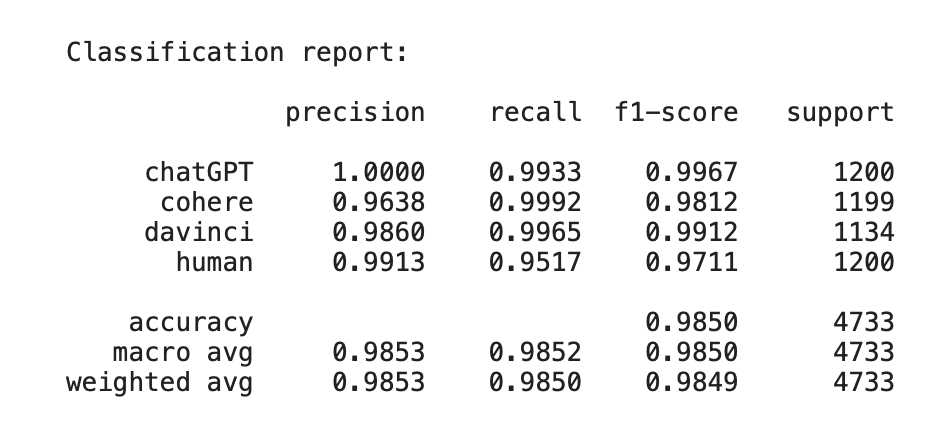
\includegraphics[width=.65\textwidth]{images/exp1_report.png}
    \caption{результат эксперимента 1}
    \label{fig:1}
\end{figure}


\newpage
\subsection{Эксперимент (2)}
\textbf{Предобученная модель DRoBERTa-base с использованием LoRA обучилась на всем обучающем датасете.}\\ \\
\begin{text}
 trainable params: 685828 all params: 82807304 || trainable\%: 0.8282    
\end{text}
Только 0.828\% параметров обучаются при использовании LoRA\\ 
\textbf{train\_runtime: 3210.977}\\
\begin{figure}[h]
    \centering
    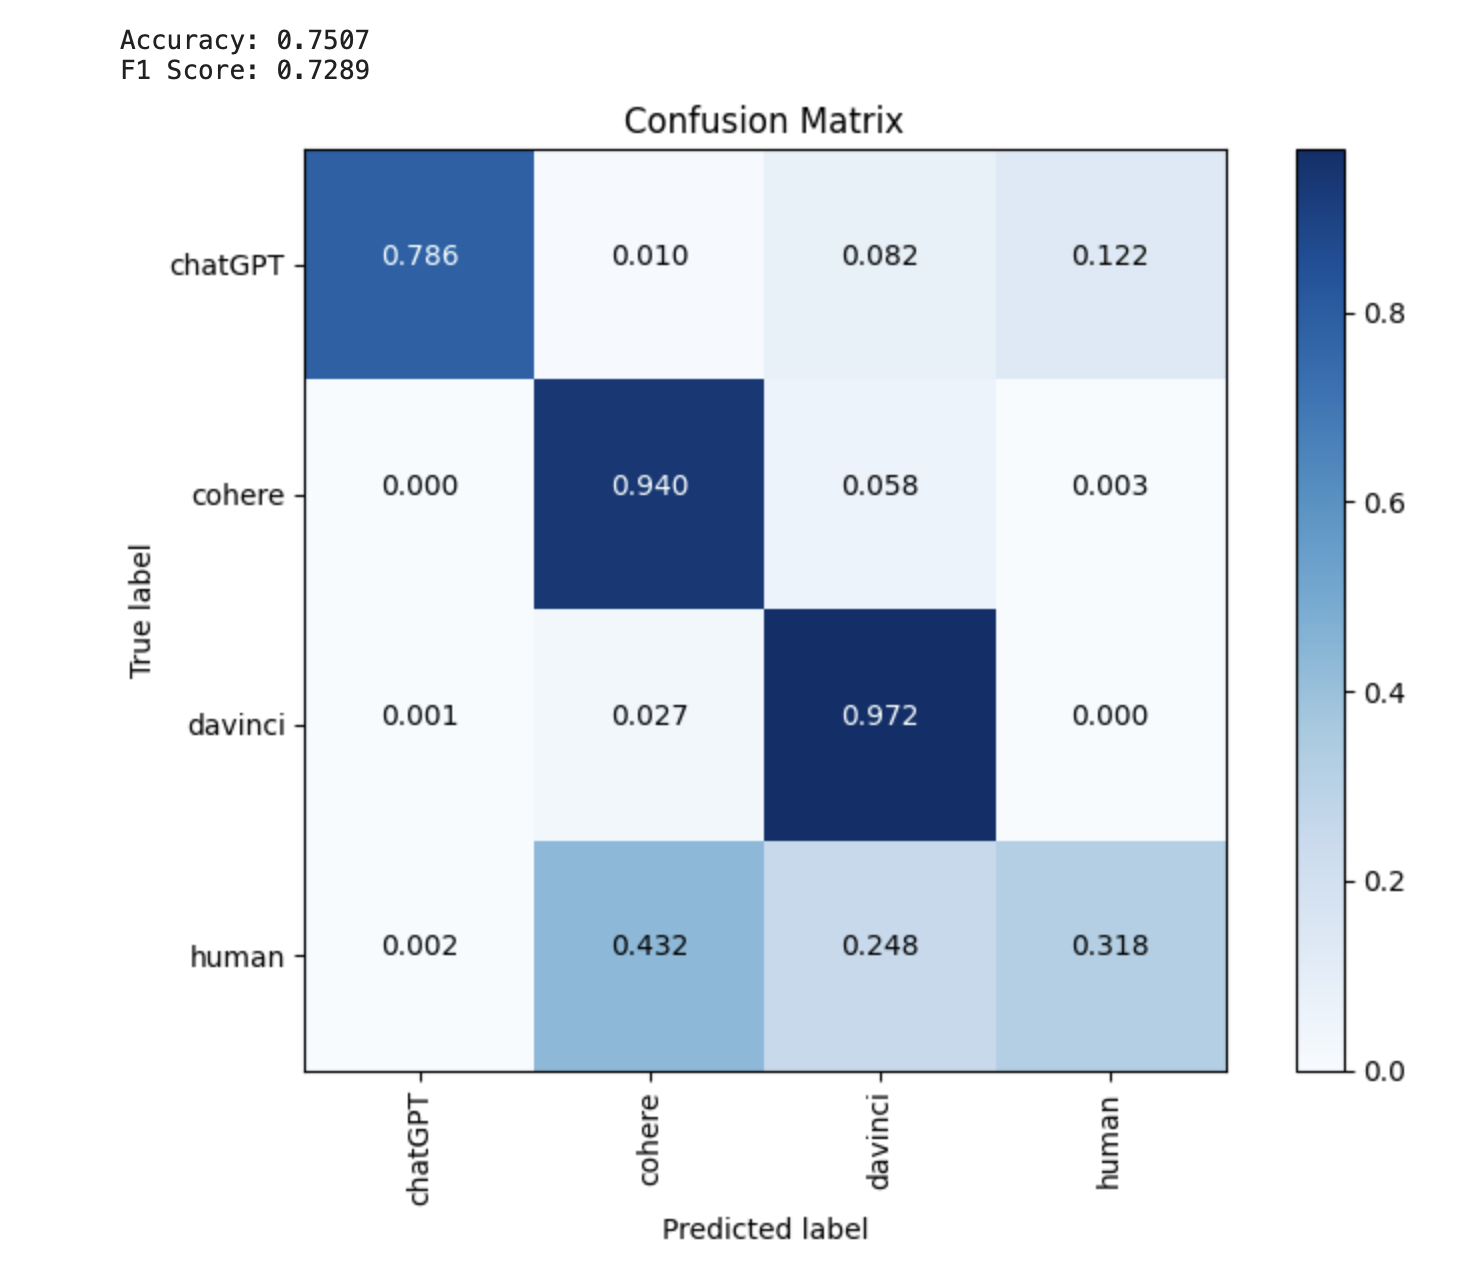
\includegraphics[width=.75\textwidth]{images/bert_lora_4.png}
    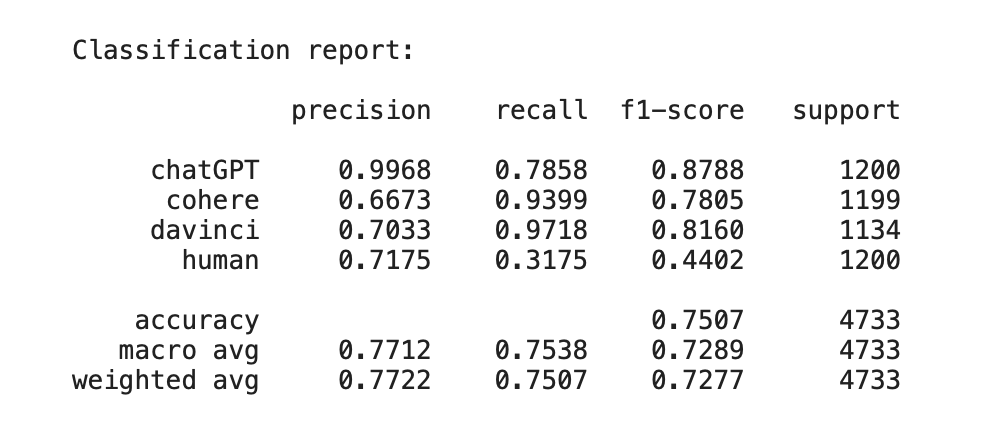
\includegraphics[width=.65\textwidth]{images/exp2_report.png}
    \caption{результат эксперимента 2}
    \label{fig:2}
\end{figure}

\newpage
\subsection{Эксперимент (3)}
\textbf{Три независимые модели DRoBERTa-base с исп. LoRA обучались на парах классов: GPT vs Human, Davinci vs Human, Cohere vs Human.}\\ \\
\textbf{ChatGPT vs Human}\\
\textbf{train\_runtime: 1633.8114}
\begin{figure}[h]
    \centering
    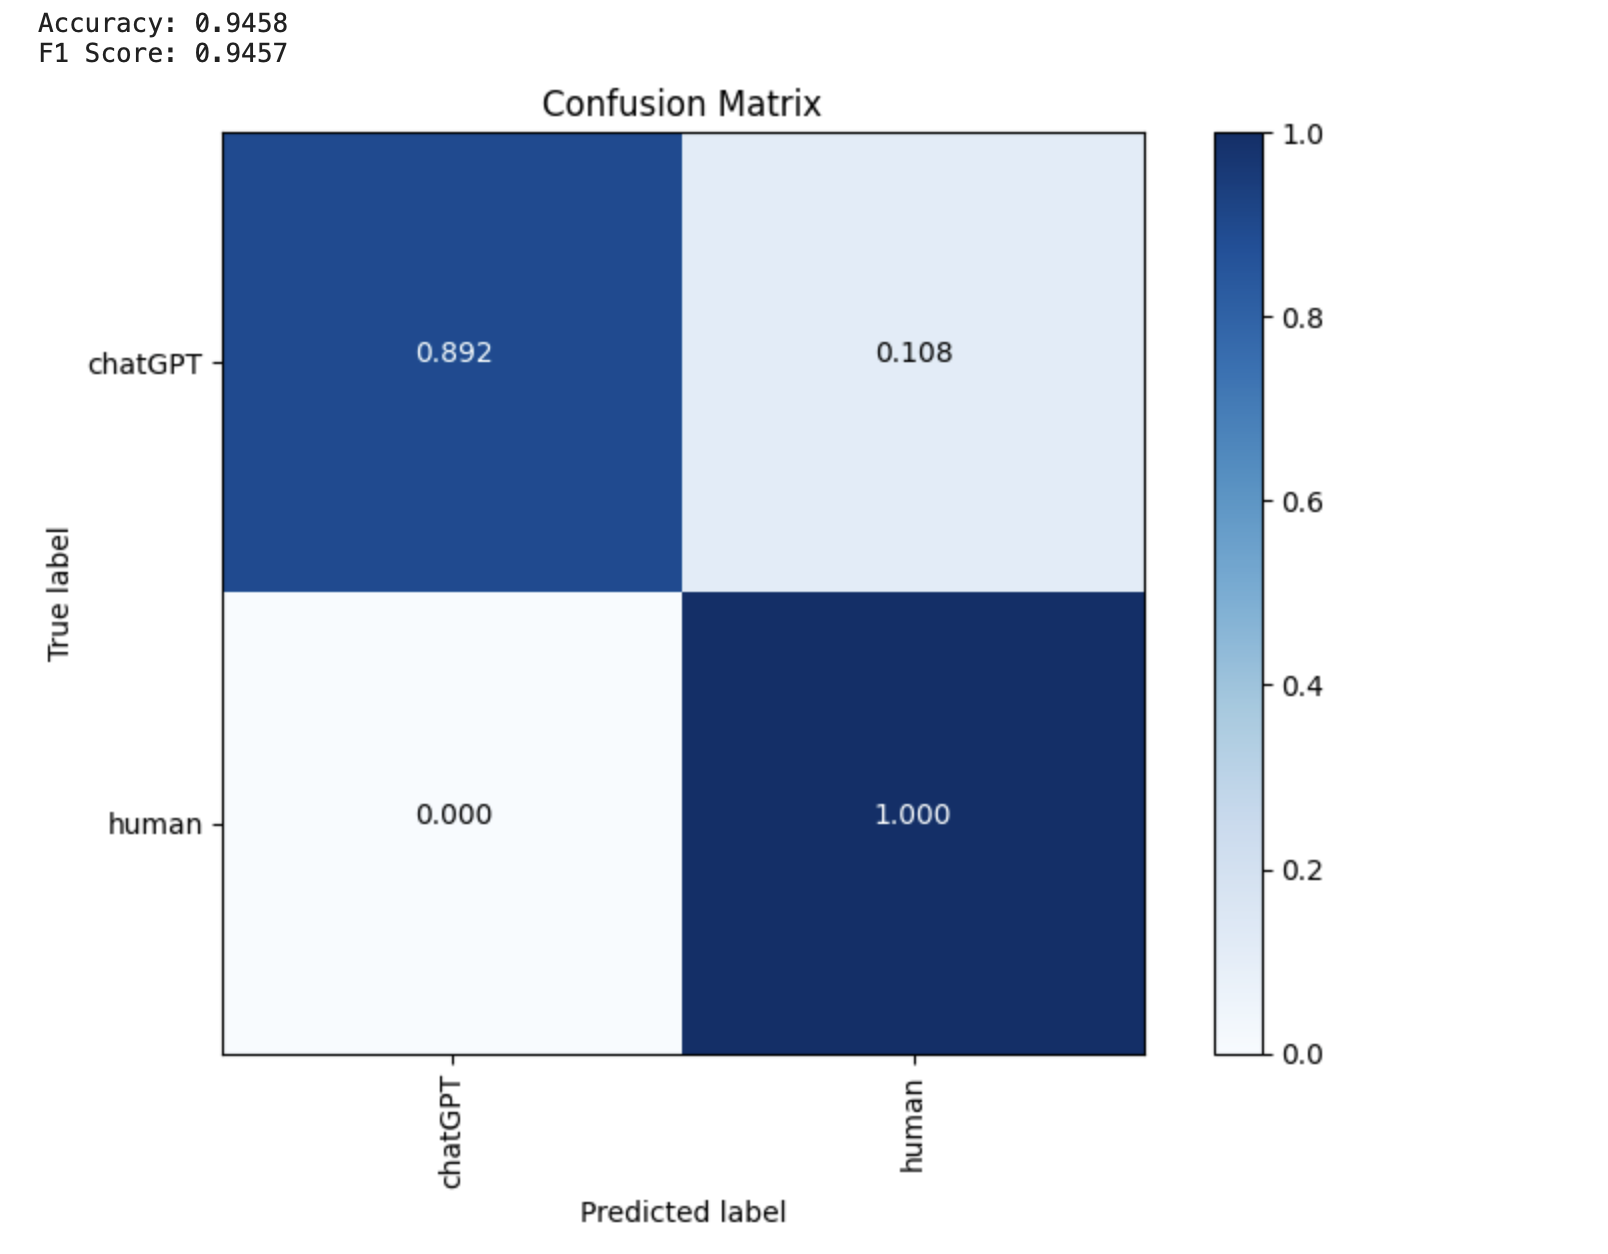
\includegraphics[width=.75\textwidth]{images/chatGPT_human.png}
    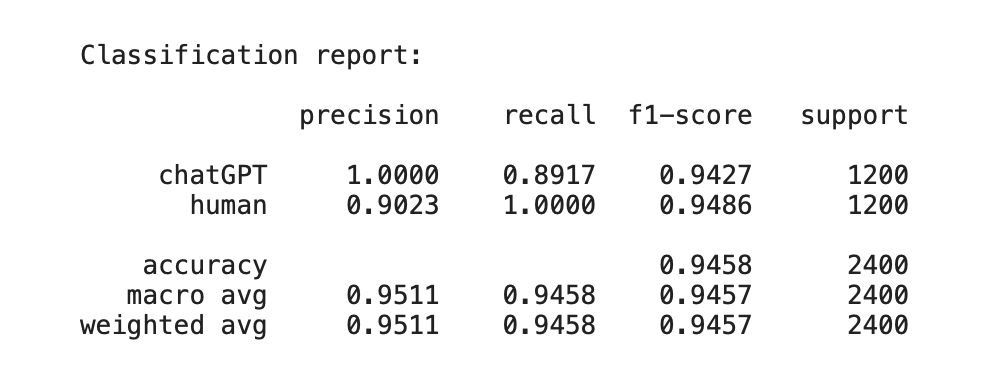
\includegraphics[width=.65\textwidth]{images/exp3_gpt.png}
    \caption{результат эксперимента 3.1}
    \label{fig:3}
\end{figure}

\newpage
\textbf{Cohere vs Human}\\
\textbf{train\_runtime: 1583.556}
\begin{figure}[h]
    \centering
    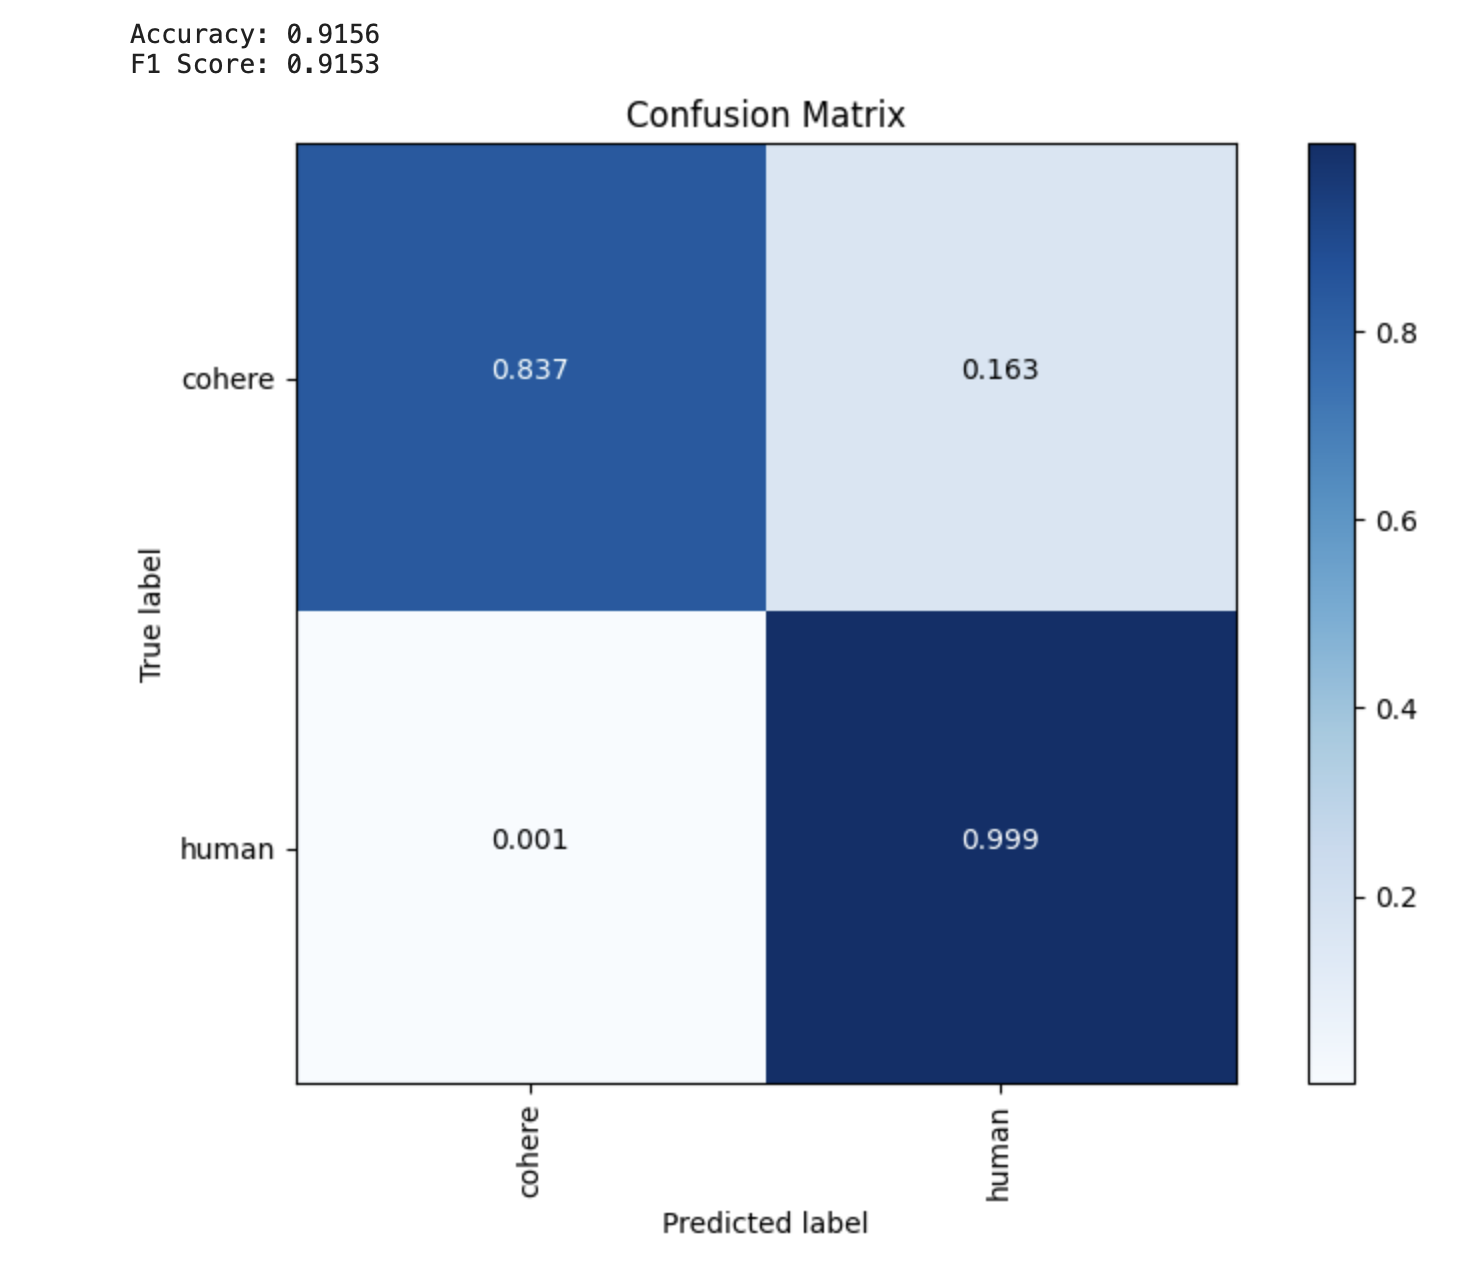
\includegraphics[width=.75\textwidth]{images/cohere_human.png}
    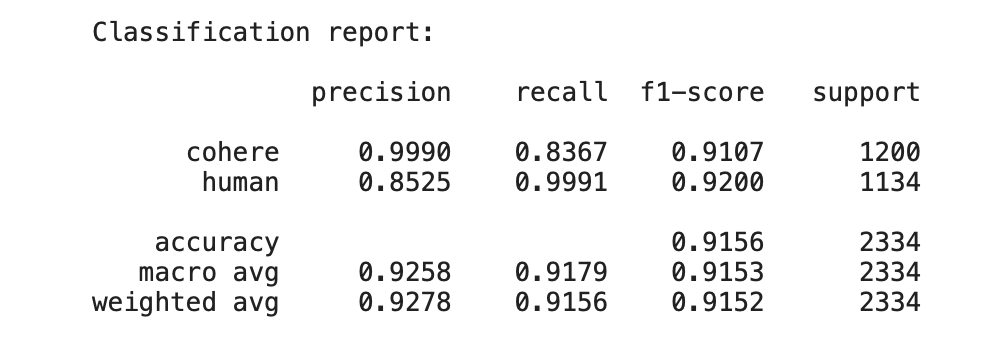
\includegraphics[width=.65\textwidth]{images/exp3_cohere.png}
    \caption{результат эксперимента 3.2}
    \label{fig:4}
\end{figure}

\newpage
\textbf{Davinci vs Human}\\
\textbf{train\_runtime: 1632.395}
\begin{figure}[h]
    \centering
    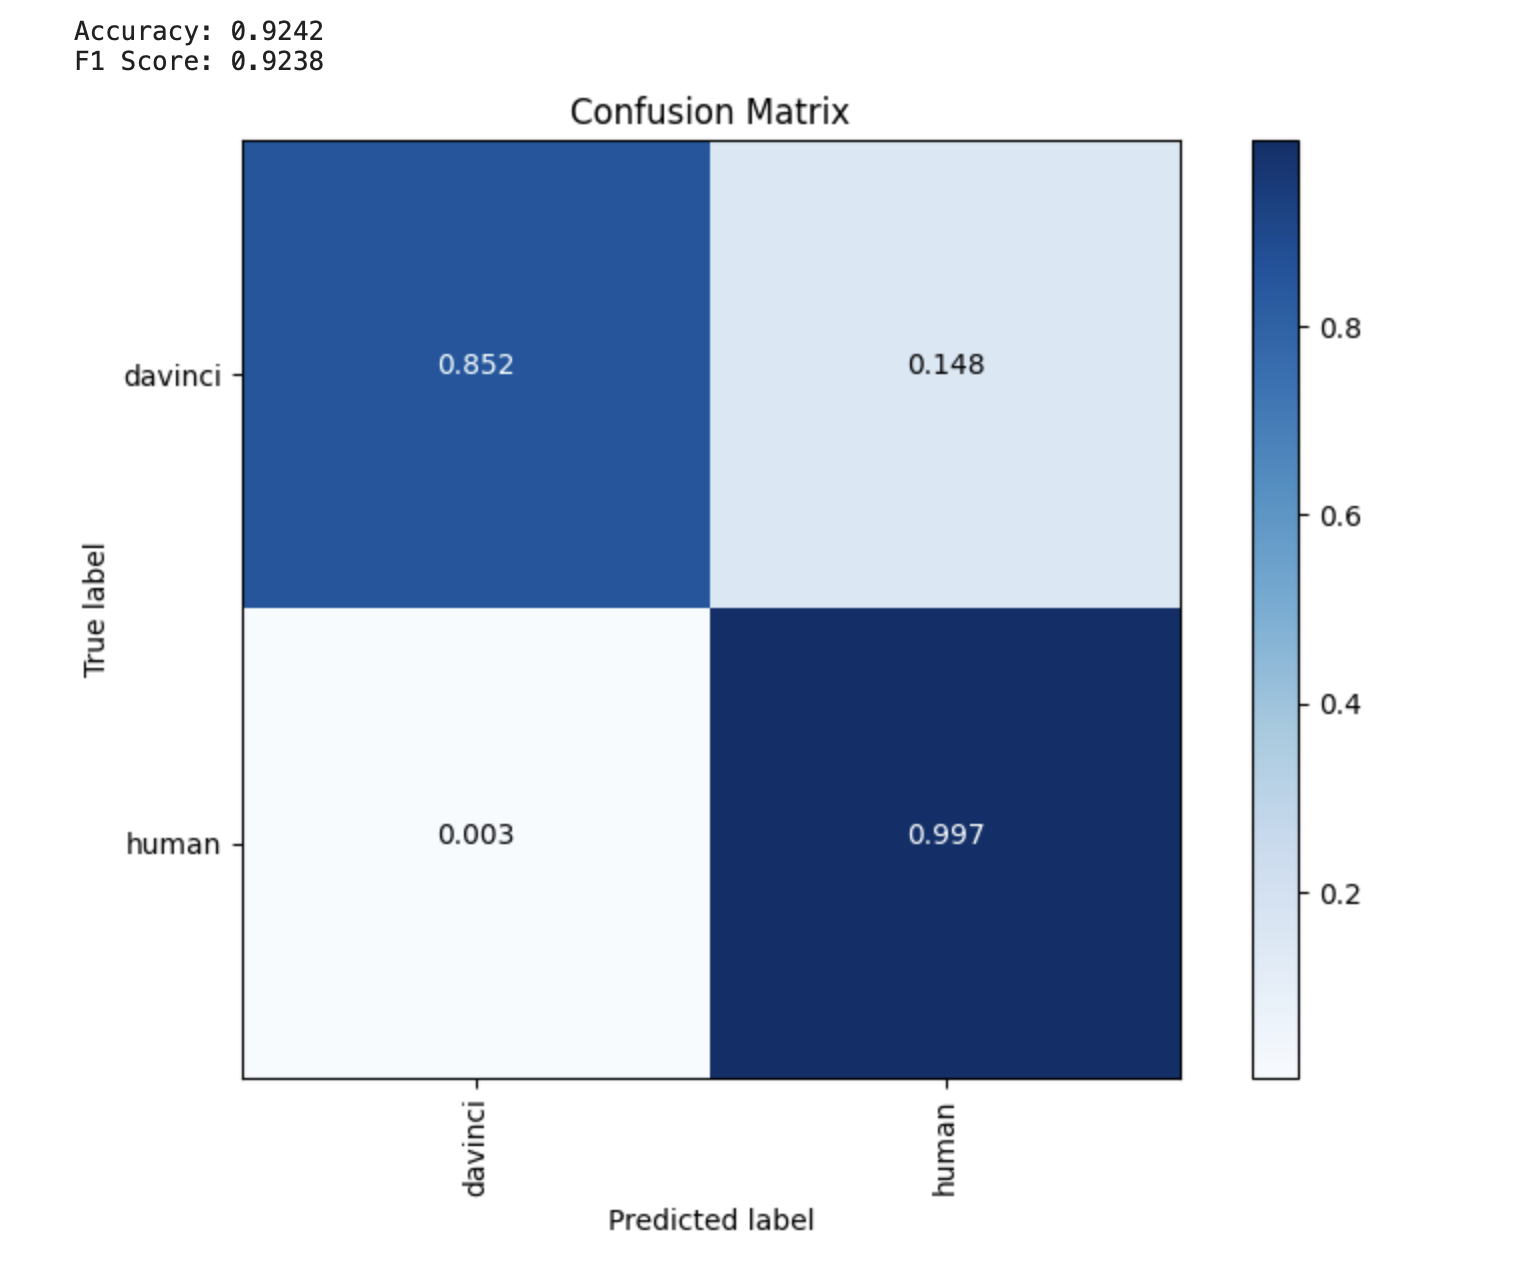
\includegraphics[width=.75\textwidth]{images/davinci_human.png}
    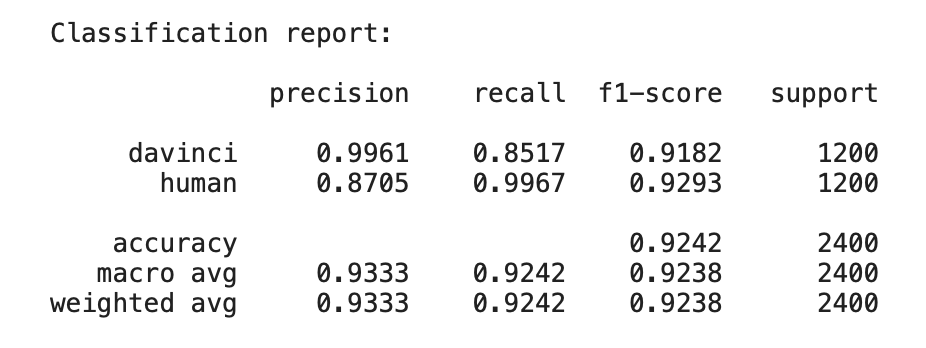
\includegraphics[width=.65\textwidth]{images/exp3_davinci.png}
    \caption{результат эксперимента 3.3}
    \label{fig:5}
\end{figure}





